\documentclass{article}

\usepackage{graphicx}
\usepackage{tikz}
\usepackage{tikzsymbols}
\usetikzlibrary{calc,patterns,shapes.geometric}
\pagestyle{empty}
\usepackage[margin=0pt]{geometry}
\geometry{papersize={14in,12in}}

\def\centerarc[#1](#2)(#3:#4:#5){\draw[#1] ($(#2)+({#5*cos(#3)},{#5*sin(#3)})$) arc (#3:#4:#5);}

\begin{document}
	\begin{figure}
		\centering
		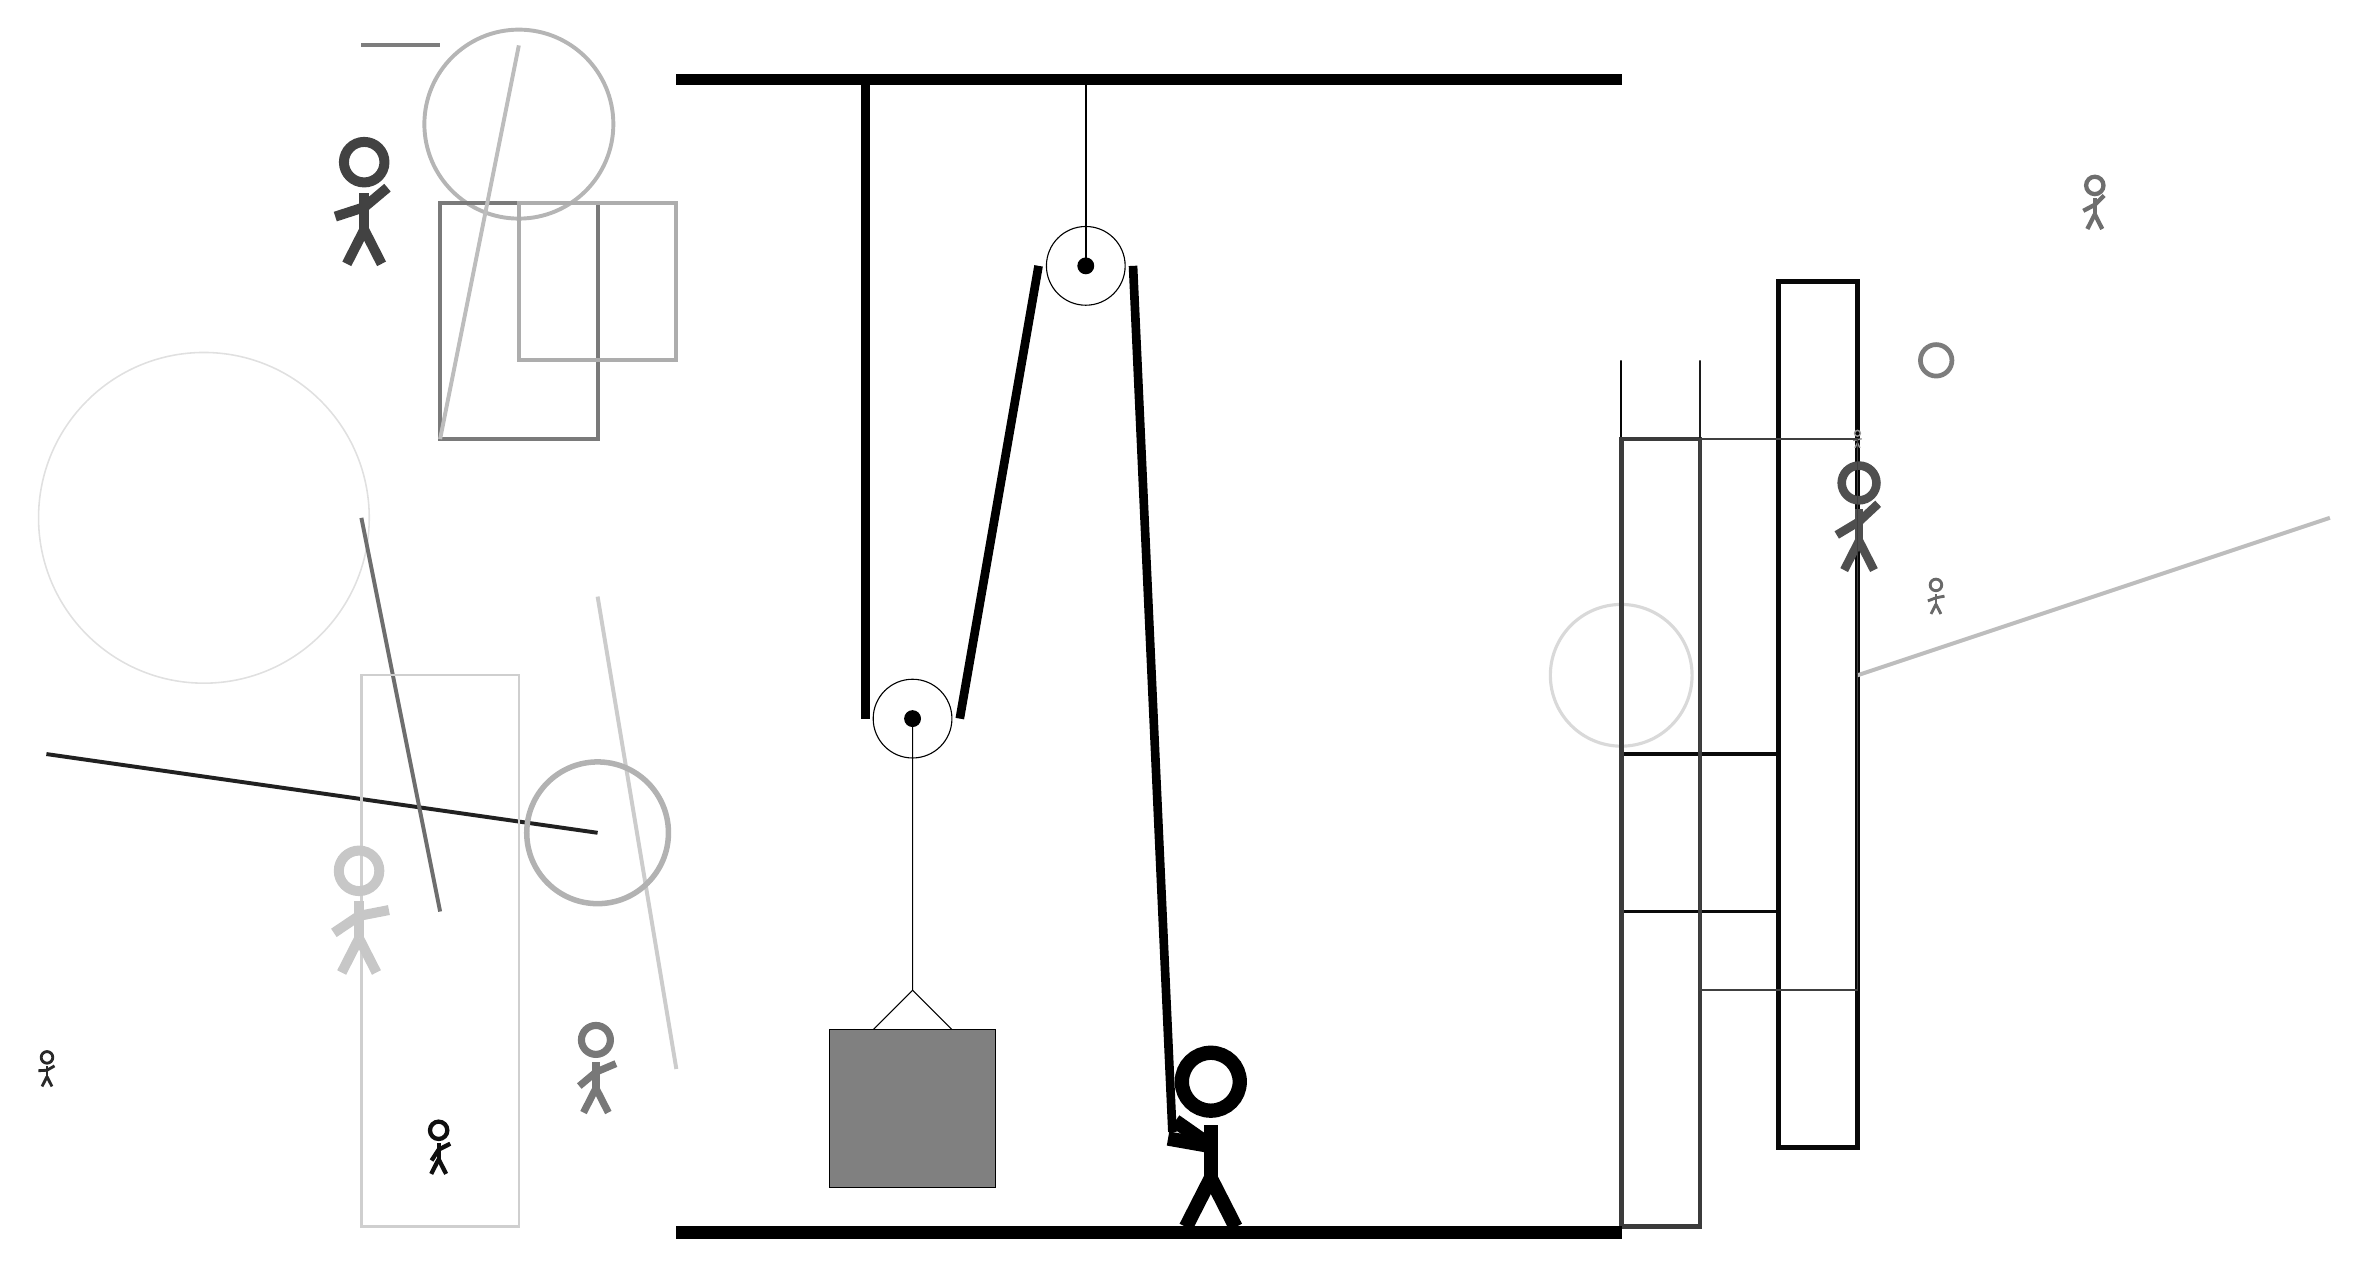
\begin{tikzpicture}
			%%%%% START %%%%%
			
			\draw[fill=black] (-2, 11.5) rectangle (10, 11.625);
			
			\draw (3.2, 9.2) circle (0.5);
			\draw[fill=black] (3.2, 9.2) circle (0.1);
			\draw[thick] (3.2, 9.2) -- (3.2, 11.5);
			
			\draw [line width=0.5mm, color=black!29](-4, 11) circle (1.2);
			
			\node[line width=0.7mm, color=black!53] at (-3, -1) {\Strichmaxerl[5][40][23]};
			\draw[line width=0.5mm, color=black!87](-3, 2) -- (-10, 3);
			\draw[line width=0.2mm, color=black!98] (10, 8) rectangle (10, -2);
			
			\draw[line width=0.5mm, color=black!52] (-3, 10) rectangle (-5, 7);
			\draw[line width=0.5mm, color=black!20](-2, -1) -- (-3, 5);
			\draw[line width=0.2mm, color=black!66] (11, 1) rectangle (12, 1);
			\node[line width=0.2mm, color=black!74] at (-6, 10) {\Strichmaxerl[7][18][40]};
			\draw [line width=0.4mm, color=black!15](10, 4) circle (0.9);
			\draw[line width=0.5mm, color=black!32] (-2, 8) rectangle (-4, 10);
			\draw [line width=0.2mm, color=black!12](-8, 6) circle (2.1);
			\node[line width=0.2mm, color=black!57] at (16, 10) {\Strichmaxerl[3][28][45]};
			\draw[line width=0.5mm, color=black!57](-6, 6) -- (-5, 1);
			\draw[line width=0.5mm, color=black!96] (10, 1) rectangle (12, 3);
			\draw[line width=0.5mm, color=black!51](-6, 12) -- (-5, 12);
			\node[line width=0.3mm, color=black!84] at (-10, -1) {\Strichmaxerl[2][3][30]};
			
			\draw[line width=0.6mm, color=black!77] (10, -3) rectangle (11, 7);
			
			\draw[line width=0.3mm, color=black!19] (-4, -3) rectangle (-6, 4);
			\draw[line width=0.6mm, color=black!97] (12, 9) rectangle (13, -2);
			\draw[line width=0.5mm, color=black!26](13, 4) -- (19, 6);
			\node[line width=0.3mm, color=black!59] at (14, 5) {\Strichmaxerl[2][21][11]};
			
			\draw [line width=0.7mm, color=black!30](-3, 2) circle (0.9);
			
			\node[line width=0.4mm, color=black!69] at (13, 6) {\Strichmaxerl[6][31][43]};
			\draw[line width=0.5mm, color=black!26](-4, 12) -- (-5, 7);
			\node[line width=0.2mm, color=black!41] at (13, 7) {\Strichmaxerl[1][9][13]};
			
			\node[line width=0.2mm, color=black!22] at (-6, 1) {\Strichmaxerl[7][34][11]};
			\draw [line width=0.6mm, color=black!51](14, 8) circle (0.2);
			\node[line width=0.3mm, color=black!94] at (-5, -2) {\Strichmaxerl[3][57][27]};
			\draw[line width=0.2mm, color=black!89] (11, 6) rectangle (11, 8);
			\draw[line width=0.2mm, color=black!75] (11, 7) rectangle (13, 0);
			
			\draw (1, 3.45) circle (0.5);
			\draw[fill=black] (1, 3.45) circle (0.1);
			
			\draw (1, 3.45) -- (1, 0.0) -- (0.5, -0.5);
			\draw (1, 0.0) -- (1.5, -0.5);
			\draw[fill=black!50] (-0.05, -0.5) rectangle (2.05, -2.5);
			
			\draw[line width=1.1mm] (0.4, 11.5) -- (0.4, 3.45);
			\centerarc[line width=1.1mm](1, 3.45)(180:360:0.6);
			\draw[line width=1.1mm](1.6, 3.45) -- (2.6, 9.2);
			\centerarc[line width=1.1mm](3.2, 9.2)(0:180:0.6);
			\draw[line width=1.1mm](3.8, 9.2) -- (4.3, -1.8);
			
			\node at (4.7, -1.9) {\Strichmaxerl[10][-35][170]};
			
			\draw[fill=black] (-2, -3) rectangle (10, -3.15);
			
			%%%%% END %%%%%
		\end{tikzpicture}
	\end{figure}	
\end{document}